\documentclass[10pt]{beamer}
% \documentclass[handout,10pt]{beamer}
\usepackage{my_style}

\title[Math/CS 375]{Lecture 15 - B}
\subtitle{\S 7.1, 7.2, 7.3 Systems of Differential Equations}

\begin{document}
% -------------------------------------------------
\begin{frame}
  \titlepage
\end{frame}
% -------------------------------------------------
\begin{frame}{Goals}
We will answer these questions:\\[3mm]
\begin{itemize}

    \item How can you use Euler's method to solve a higher order IVP?
    
    \item What is the main idea behind the Runge-Kutta methods?
    
    \item How do we update all components of a coupled system?
\end{itemize}
\end{frame}




%%%%%%%%%%%%%%%%%%%%%%%%%%%%%%%%%%%%%%%%%%%%
\sectionframe{System of ODEs}
%%%%%%%%%%%%%%%%%%%%%%%%%%%%%%%%%%%%%%%%%%%%

\begin{frame}[shrink]{Population Model}

\begin{block}{Rabbits}
Let $R(t)$ = population of rabbits at time $t$. Then we can model their population as
$$
    R' = cR 
$$
where $c>0$ is some growth rate constant. 
\begin{itemize}
    \item If $R$ is small, then population increase rate $R'$ is small.
    \item If $R$ is big, then population increase rate $R'$ is big.
    \item Idea: more rabbits $\implies$ more breeding
\end{itemize}    
\end{block}

\onslide<2->{
\begin{block}{Foxes}
Let $F(t)$ = population of foxes at time $t$ and model it as 
$$
    F' = -k F
$$
where $k>0$.
\begin{itemize}
    \item Food is very scarce and they are dying out
    \item Assume a constant per-capita death rate $k$ in the absence of prey
\end{itemize}
\end{block}
}
\end{frame}


\begin{frame}{Rabbits and Foxes}

\begin{figure}
    \centering
    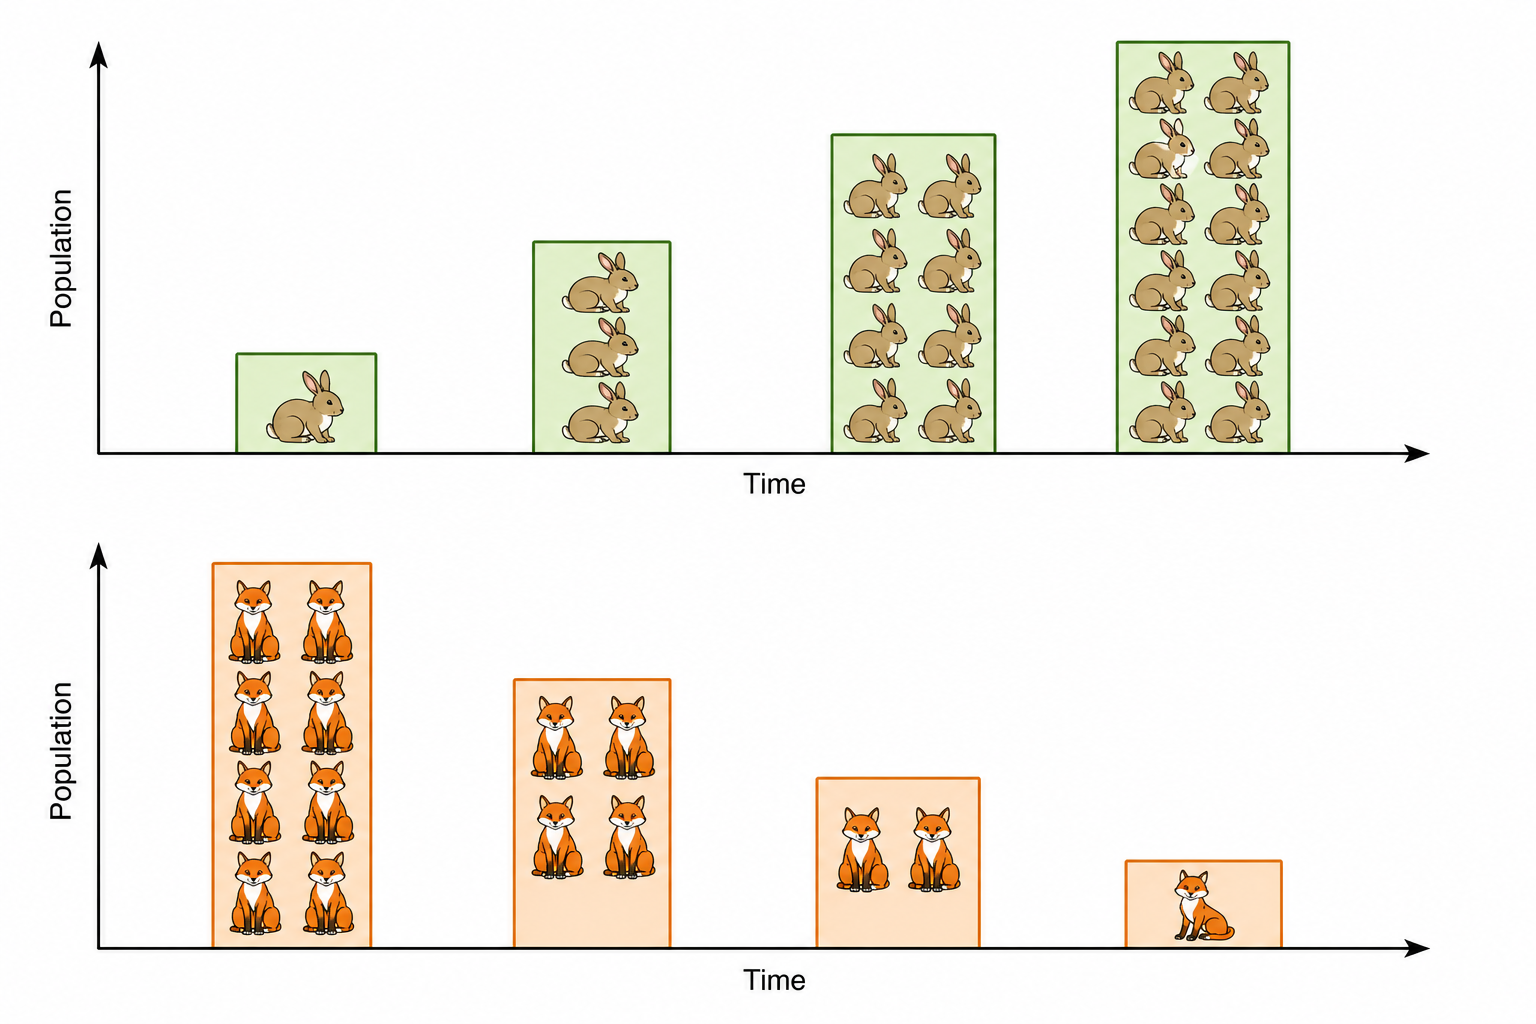
\includegraphics[width=0.8\linewidth]{figs/rabbits_foxes.png}
\end{figure}
\begin{itemize}
    \item Rabbits have infinite amount of grass to graze on 
    \item Foxes have little/no food available
\end{itemize}
\end{frame}

% ------------------
\begin{frame}{Predator-Prey Model}

{
\question{What if both Foxes and Rabbits lived in the same niche?}
}

\begin{itemize}

    \item Then Rabbits = Food for Foxes

    \begin{block}{Predator-Prey Model}
    \[
    \begin{cases}
    R^\prime = cR - RF, & \quad \text{Prey growth rate}\\
    F^\prime = RF - kF, & \quad\text{Predator growth rate}
    \end{cases}
    \]
    \begin{itemize}
        \item Population of rabbits and foxes influence each other
        \item The term $RF$ represents how often they encounter each other
        \item Idea: Foxes prey on Rabbits 
        \item This is a \textbf{system of ODEs}
    \end{itemize}
    \end{block}

\end{itemize}
\end{frame}

%%%%%%%%%%%%%%%%%%%%%%%%%%%%%%%%%%%%%%%%%%%%
\begin{frame}{Predator and Prey}
\begin{figure}
    \centering
    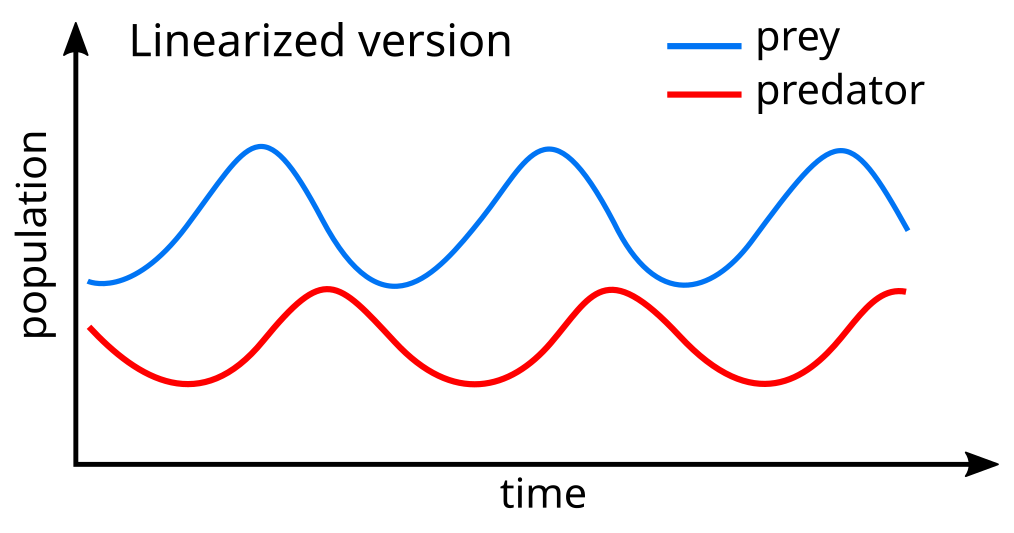
\includegraphics[width=0.7\linewidth]{figs/Lotka_Volterra_dynamics.png}
    % \caption{https://en.wikipedia.org/wiki/Lotka-Volterra\_equations}
\end{figure}
    
    \begin{block}{Goal}
       Learn about \textbf{systems of ODEs} and how to numerically solve them using Euler's method.
   \end{block}
\end{frame}

%%%%%%%%%%%%%%%%%%%%%%%%%%%%%%%%%%%%%%%%%%%%

\begin{frame}{Coupled System}
\begin{itemize}
\item Suppose you had a \textbf{coupled system}  
\[
\begin{cases}
u_1^\prime(t) = f_1(t,u_1,u_2), \qquad u_1(0) = a \\
u_2^\prime(t) = f_2(t,u_1,u_2), \quad \quad \, u_2(0) = b 
\end{cases}
\]
\item $u_1$ and $u_2$ depend on each other so we solve for them together 
\item Discretize time $t_i = ih$, with $h=T/n$ on $[0,T]$

\item We seek discrete solutions of $u_1(t)$ and $u_2(t)$
\[
\mathbf{u_1} = 
\begin{bmatrix} 
\textbf{u}_{1,0} \\ 
\textbf{u}_{1,1} \\ 
\vdots \\  
\textbf{u}_{1,n} 
\end{bmatrix}
\approx  
\begin{bmatrix} 
u_1(t_0) \\ 
u_1(t_0 + h) \\ 
\vdots \\  
u_1(t_0 + nh) 
\end{bmatrix},
\quad
\mathbf{u_2} = 
\begin{bmatrix} 
\textbf{u}_{2,0} \\ 
\textbf{u}_{2,1} \\ 
\vdots \\  
\textbf{u}_{2,n} 
\end{bmatrix}
\approx  
\begin{bmatrix} 
u_2(t_0) \\ 
u_2(t_0 + h) \\ 
\vdots \\  
u_2(t_0 + nh) 
\end{bmatrix}.
\]

\end{itemize}
\end{frame}
%%%%%%%%%%%%%%%%%%%%%%%%%%%%%%%%%%%%%%%%%%%%
\begin{frame}{Use Taylor Expansion}


\begin{itemize}
    \item Taylor-expand both solutions
    \begin{align*}        
    u_1(t_i+h) &\approx u_1(t_i) + h u_1'(t_i) \\
           &= u_1(t_i) + h f_1(t_i, u_1(t_i),u_2(t_i))\\[3mm]
    u_2(t_i+h) &\approx u_2(t_i) + h u_2'(t_i) \\
           &= u_2(t_i) + h f_2(t_i, u_1(t_i),u_2(t_i))
    \end{align*}

    \item For the first component, the time-stepping rule is
        $$
        \textbf{u}_{1,i+1} = \textbf{u}_{1,i} + h\,f_1(t_i, \textbf{u}_{1,i},\textbf{u}_{2,i} )
        $$
    \item This is \textbf{Euler's Method for a coupled system}
\end{itemize}

\end{frame}
% -----------------
\begin{frame}{Euler's Method for Coupled Systems}
\begin{itemize}
    \item System to solve:
    \[
    \begin{cases}
    u_1^\prime = f_1(t,u_1,u_2), \qquad u_1(0) = a \\
    u_2^\prime = f_2(t,u_1,u_2), \quad \quad \, u_2(0) = b
    \end{cases}
    \]

    \item Euler's method for systems
    \[
    \begin{cases}
    \textbf{u}_{1,i+1} = \textbf{u}_{1,i} + h \cdot f_1(t_i, \textbf{u}_{1,i}, \textbf{u}_{2,i}), \\
    \textbf{u}_{2,i+1} = \textbf{u}_{2,i} + h \cdot f_2(t_i, \textbf{u}_{1,i}, \textbf{u}_{2,i}).
    \end{cases}
    \]

    \keyidea{
    Compute both new values using the same old pair. Do not overwrite one component before updating the other.
    }

\end{itemize}
\end{frame}


%%%%%%%%%%%%%%%%%%%%%%%%%%%%%%%%%%%%%%%%%%%

\begin{frame}{Euler Example for a System}{Part 1}
\begin{example}
Apply Euler's method with $h = 0.5$ to the IVP
\[
\begin{cases}
u_1' = u_2, \\
u_2' = -u_1, \\
u_1(0) = 1, \quad u_2(0) = 0
\end{cases}
\]
over the time interval $t \in [0, 1]$.
\end{example}

\begin{itemize}
    \item Step 1: step from $t=0$ to $t=0.5$
    \begin{align*}
    u_1(0.5) &\approx u_1(0.0) + h \cdot f_1( u_1(0.0), u_2(0.0)) = 1 + 0.5*(0) = 1,\\
    u_2(0.5) &\approx u_2(0.0) + h \cdot f_2(u_1(0.0),u_2(0.0)) = 0 + 0.5*(-1) = -0.5
    \end{align*}

\end{itemize}
\end{frame}


%%%%%%%%%%%%%%%%%%%%%%%%%%%%%%%%%%%%%%%%%%%

\begin{frame}{Euler Example for a System}{Part 2}


\begin{itemize}
    \item Step 1: 
    \begin{align*}
    u_1(0.5) &\approx 1,\\
    u_2(0.5) &\approx  -0.5
    \end{align*}
    
    \item Step 2: formula step from $t=0.5$ to $t=1.0$
    \begin{align*}
    u_1(1.0) &\approx u_1(0.5) + h \cdot f_1( u_1(0.5), u_2(0.5))\\
    u_2(1.0) &\approx u_2(0.5) + h \cdot f_2(u_1(0.5),u_2(0.5)) 
    \end{align*}
    \item Substitute and evaluate
    \begin{align*}
    u_1(1.0) &\approx 1 + 0.5 \cdot (-0.5) = 0.75 \\
    u_2(1.0) &\approx -0.5 + 0.5\cdot(-1) = -1.0
    \end{align*}
\end{itemize}
\end{frame}


%-------------------------------------------
\begin{frame}{Rabbits and Foxes}
    \begin{block}{Model}
        Let $x(t)=$ population of rabbits and $y(t)=$population of foxes (in hundreds at $t$ months).
        $$
        \begin{dcases}
            x' = 4x -2xy\\
            y' = -3y + xy
        \end{dcases}
        $$
        There are initially 300 rabbits and 400 foxes.
    \end{block}
    \begin{itemize}
        \item This is a system of the form 
        $$
        \begin{dcases}
            x' =f_1(x,y)\\
            y' = f_2(x,y)
        \end{dcases}
        $$
        so we can use \textit{Euler's method} to solve this equation
    \end{itemize}
    
\end{frame}
%-------------------------------------------
\begin{frame}{Applying Euler's Method}
\begin{itemize}
    \item Discretize time $\{t_0,t_1,\dots,t_n\}$
    
    \item Create two discrete vectors for rabbit and fox populations
    $$
    \textbf{x} = \begin{bmatrix}
        3\\0\\\vdots\\0
    \end{bmatrix}, \quad \textbf{y} = \begin{bmatrix}
        4\\0\\\vdots\\0
    \end{bmatrix}
    $$
    \item Then iterate for $i$ from $0$ to $n-1$ 
    \begin{align*}    
    x_{i+1} = x_i+h( 4x_i-2x_iy_i)\\ 
    y_{i+1} =y_i+h(-3y_i+x_iy_i)
    \end{align*}

    \item There are two Ways to visualize the solution
\end{itemize}
\end{frame}

%-------------------------------------------
\begin{frame}{Two Ways to Visualize the Solution}
\cols{
\begin{figure}
    \centering
    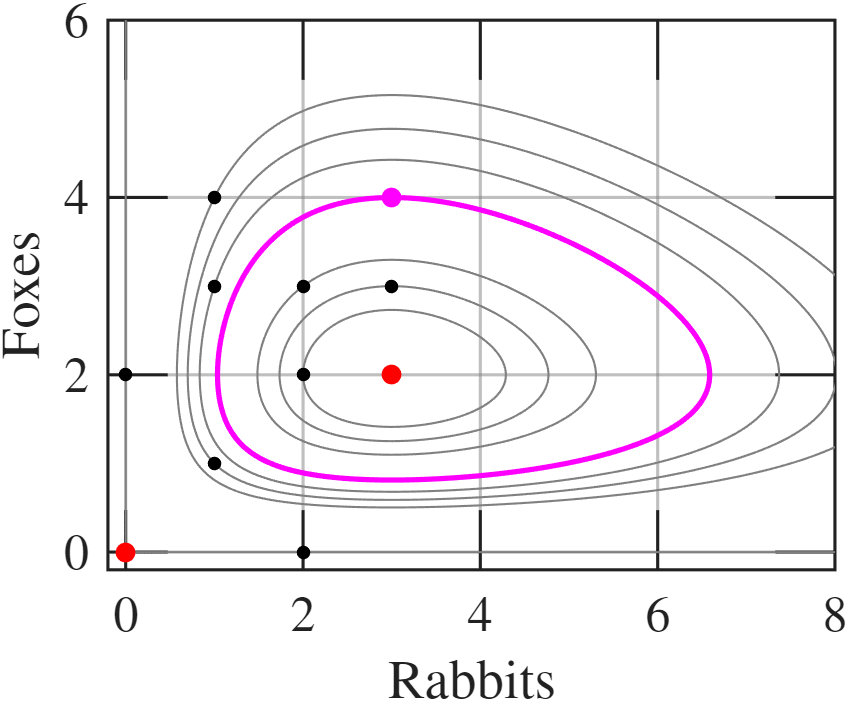
\includegraphics[width=\linewidth]{figs/rf1.png}
    \caption{\texttt{plot(x,y)}}
\end{figure}
}{
\begin{figure}
    \centering
    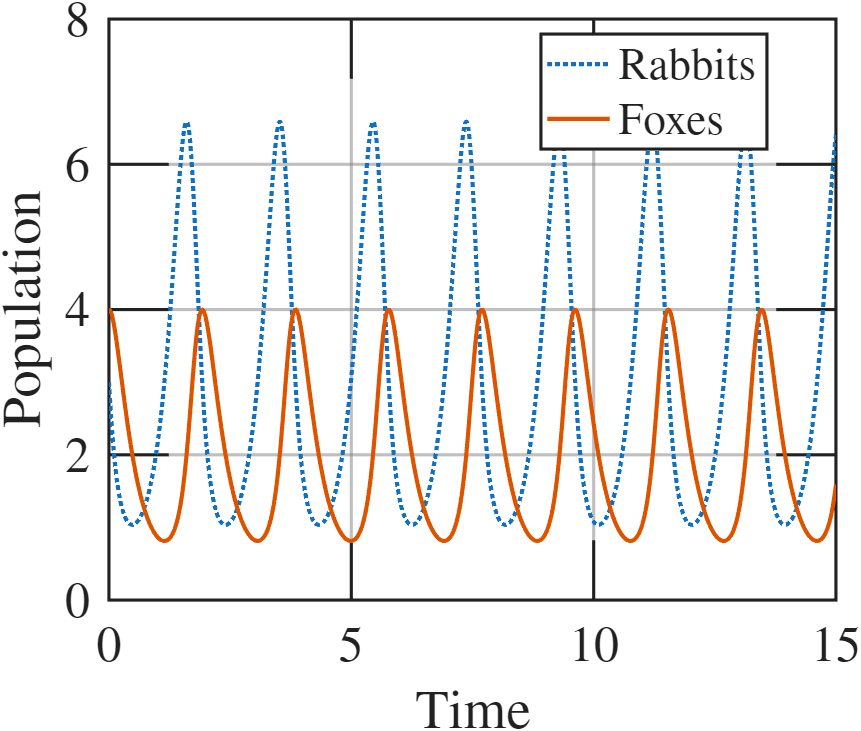
\includegraphics[width=\linewidth]{figs/rf2.png}
    \caption{\texttt{plot(t,x,t,y)}}
\end{figure}
}
\begin{block}{Interpretation}
    The ideal model has periodic cycles for positive, non-equilibrium initial populations. Euler approximations can drift over time. 
\end{block}
\end{frame}
%-------------------------------------------
%-------------------------------------------
\sectionframe{General Euler's Method}
\begin{frame}{General System}
\begin{itemize}
    \item In general, a first-order system of $m$ ODEs has the form
\[
\begin{cases}
u_1^\prime = f_1(t,u_1, u_2, \ldots, u_m)\\
u_2^\prime = f_2(t,u_1, u_2, \ldots, u_m) \qquad t \in (a,b]\\
\quad \vdots \\
u_m^\prime = f_m(t,u_1, u_2, \ldots, u_m)\\
\end{cases}
\]
\item Each variable has its own initial condition:
\[
\begin{cases}
u_1(a) = u_{1a}\\
u_2(a) = u_{2a}\\
\quad \vdots\\
u_m(a) = u_{ma}\\
\end{cases}
\]
\end{itemize}
\end{frame}
%%%%%%%%%%%%%%%%%%%%%%%%%%%%%%%%%%%%%%%%%%%%
\begin{frame}{Compact Notation}
\begin{itemize}
    \item It may be cumbersome to write 
    $$
    \begin{cases}
    u_1^\prime = f_1(t,u_1, u_2, \ldots, u_m)\\
    \quad \vdots \\ 
    u_m^\prime = f_m(t,u_1, u_2, \ldots, u_m)\\
    \end{cases}\qquad t \in (a,b]
    $$
    \item So we introduce a vector function $\mathbf{u}(t)$ to be the mapping $\mathbf{u}:\mathbb{R}\rightarrow \mathbb{R}^{m}$
    $$
        \mathbf{u}(t) = 
        \begin{bmatrix} 
        u_{1}(t) & \cdots &  u_{m}(t) 
        \end{bmatrix}^T
    $$
    \item Let 
    $$
        \mathbf{F}(t,\textbf{u}) = 
        \begin{bmatrix} 
        f_1(t,\textbf{u}) & \cdots &  f_{m}(t,\textbf{u}) 
        \end{bmatrix}^T
    $$
\end{itemize}
    
    \begin{block}{Compact Notation for a System}
    We may define $\mathbf{F}(t,\textbf{u})$ to be the compact form for $f_i$ for $i = 1$ to $m$ so that we may write the ODE as
        $$\underbrace{\mathbf{u}'(t)}_{\text{vector of derivatives}} =\;\; \underbrace{\mathbf{F}(t,\mathbf{u})}_{\text{vector of f's}}$$
    \end{block}
\end{frame}
%%%%%%%%%%%%%%%%%%%%%%%%%%%%%%%%%%%%%%%%%%%%
\begin{frame}{Euler's Method for Systems}
\begin{itemize}
    \begin{block}{Euler's Method}
        
    To solve the $m$ dimensional first-order IVP
    \[
    \mathbf{u}^\prime(t) = \mathbf{F}(t, \mathbf{u}), \quad \mathbf{u}(t_0) = \mathbf{u}_0,
    \]
    apply Euler's method component-wise:
    \[
    \mathbf{u}_{i+1} = \mathbf{u}_i + h \cdot \mathbf{F}(t_i, \mathbf{u}_i),
    \]
    where \(t_i = t_0 + i h\) and \(h\) is the step size.
    \end{block}

    \item The compact Euler's method is shorthand for
    \[
    \begin{cases}
    u_{1,i+1} = u_{1,i} + h \cdot f_1(t_i, u_{1,i}, \ldots, u_{m,i}), \\
    u_{2,i+1} = u_{2,i} + h \cdot f_2(t_i, u_{1,i}, \ldots, u_{m,i}), \\
    \quad \vdots \\
    u_{m,i+1} = u_{m,i} + h \cdot f_m(t_i, u_{1,i}, \ldots, u_{m,i}).
    \end{cases}
    \]

\end{itemize}
\end{frame}

%%%%%%%%%%%%%%%%%%%%%%%%%%%%%%%%%%%%%%%%%%%%
\begin{frame}{Time-Stepping for Any Number of Variables}
For autonomous systems (no explicit dependence on time):

\begin{block}{Euler with One Unknown}
    $$ \texttt{new} = \texttt{old} + h*f(\texttt{old})$$
\end{block}

\begin{block}{Euler with Two Unknowns}
    \begin{align*}
        \texttt{new1} &= \texttt{old1} + h*f_1(\texttt{old1},\texttt{old2})\\
        \texttt{new2} &= \texttt{old2} + h*f_2(\texttt{old1},\texttt{old2})
    \end{align*}
\end{block}

\begin{block}{
    Euler with $m$ Unknowns
}
    \begin{align*}
        \textbf{\texttt{new}} &= \textbf{\texttt{old} }+ h*\textbf{F}(\textbf{\texttt{old}})
    \end{align*}
    \textbf{\texttt{new}} and \textbf{\texttt{old}} are vectors of length $m$
\end{block}

\end{frame}


%%%%%%%%%%%%%%%%%%%%%%%%%%%%%%%%%%%%%%%%%%%%
\sectionframe{Higher Order ODEs}
%%%%%%%%%%%%%%%%%%%%%%%%%%%%%%%%%%%%%%%%%%%%

\begin{frame}{Why This Simple Method Is Useful}

% \begin{block}{First Order Problem}
%     We know Euler's method can handle any IVP of the form
%     $$
%     \begin{dcases}
%         u' = f(t,u),\quad t\in(0,T]\\
%         u(0)=u_0
%     \end{dcases}
%     $$
% \end{block}

\question{
    How far can this simple update take us?
    $$
    u_{i+1} = u_i +hf(u_i)
    $$
}



    \begin{figure}
        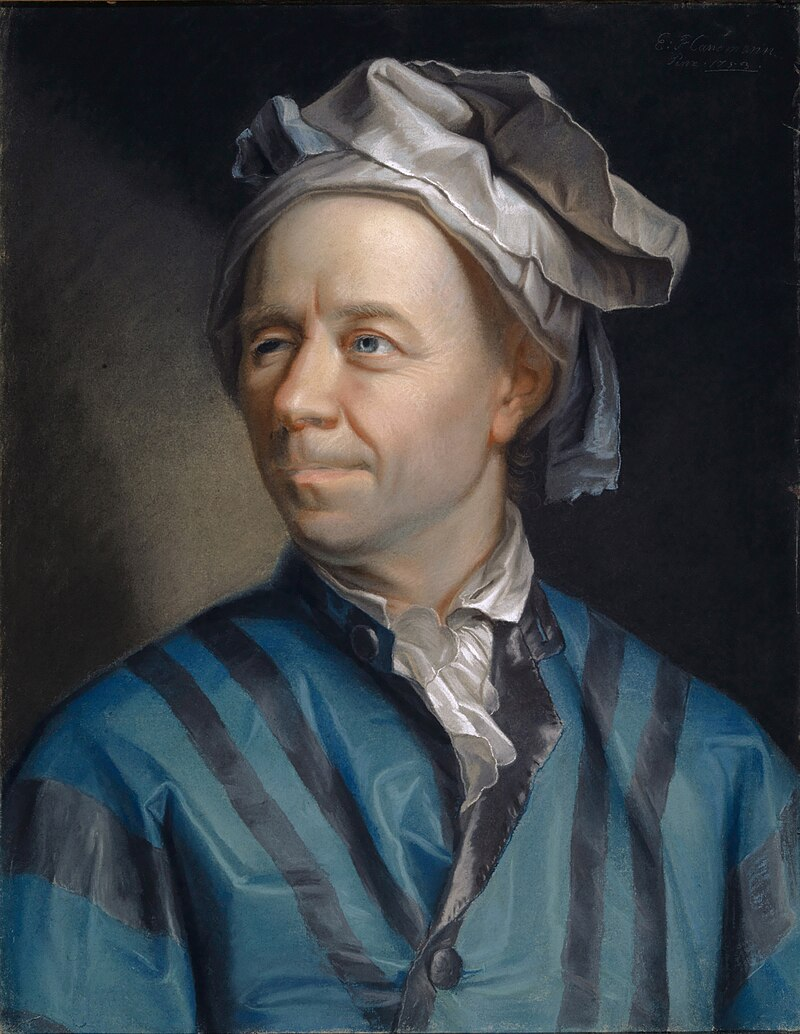
\includegraphics[scale=0.1]{figs/euler.jpg}
    \end{figure}
\onslide<2>{
\begin{center}
It also handles higher-order ODEs after rewriting them as systems.
\end{center}
}

\end{frame}

\begin{frame}{Higher-Order ODEs}
\begin{itemize}
    \item The \textbf{order} refers to the highest derivative. 
    \begin{align*}    
    \underbrace{u^{\prime}(t)}_{\text{1st order}} + 2\, u &= 6\\
    \underbrace{2u^{\prime\prime}(t)}_{\text{2nd order}} - \, u^\prime(t) + 7 \, u(t) &= 0.
    \end{align*}
    

    \item Euler’s method requires a first-order equation or system.\\[3mm]

    \item We may introduce new variables to change the ODE\\[3mm]

    \begin{block}{Goal}
        Rewrite the second-order ODE as a first-order system.
    \end{block}


\end{itemize}
\end{frame}

\begin{frame}{Introducing New Variables}
\begin{itemize}
    \item Consider the 2nd-order ODE:
    \[
    u^{\prime\prime}(t) + a u^\prime(t) + b t u(t) = c.
    \]

    \item Introduce \textit{new} variables $y_1$ and $y_2$:
    \[
    \begin{cases}
    y_1 = u(t), & \text{(the original function)}, \\
    y_2 = u^\prime(t), & \text{(the first derivative of the original)}.
    \end{cases}
    \]

    \item We may take the derivative of $y_1(t)$ and $y_2(t)$
    \[
    \begin{cases}
    y'_1 = u'(t) \\
    y'_2 = u^{''}(t) .
    \end{cases}
    \]
\end{itemize}
\end{frame}


\begin{frame}{Rewriting as a First-Order System}
\begin{itemize}
    \item Using the definitions \(y_1 = u\) and \(y_2 = u^\prime\), compute derivatives:
    \[
    \begin{cases}
    y_1^\prime = u^\prime = y_2, \\
    y_2^\prime = u^{\prime\prime}.
    \end{cases}
    \]

    \item Substitute \(u^{\prime\prime}\) from the original ODE:
    \[
    u^{\prime\prime} = -a u^\prime - b t u + c \equiv y_2^{\prime}.
    \]

\onslide<2>{
\begin{block}{Result}
    Rewrite in terms of \(y_1\) and \(y_2\):
    \[
    \begin{cases}
    y_1^\prime = y_2, \\
    y_2^\prime = -a y_2 - b t y_1 + c
    \end{cases} \;\Leftrightarrow\; 
    \begin{cases}
    y_1^\prime = f_1(t,y_1,y_2), \\
    y_2^\prime = f_2(t,y_1,y_2)
    \end{cases}
    \]
\end{block}

{
\keyidea{2nd Order DEs are the same as a 1st order system.}
}
}



\end{itemize}
\end{frame}
%%%%%%%%%%%%%%%%%%%%%%%%%%%%%%%%%%%%%%%%%%%%

\begin{frame}{Euler's Idea}

\begin{block}{Original ODE}
    $$
    \begin{cases}
    u^{''}- 2 u^\prime + 8 u  = 0, \quad t \in (0,T]\\
    u(0) = A, u^\prime(0) = B
    \end{cases}
    $$
\end{block}

\begin{block}{New Equivalent System}
    \[
    \begin{cases}
    y_1^\prime = y_2, \\
    y_2^\prime = -8u+2u'=-8y_1+2y_2\\
    y_1(0)=A,\;\; y_2(0)=B
    \end{cases}
    \]
\end{block}

Euler's Idea:
\begin{itemize}
    \item Euler's update does not directly apply to the second-order form
    \item Rewrite the ODE as a first-order system 
    \item Now apply Euler to approximate both components 
    \item The solution to the original problem is $y_1(t) = u(t)$
\end{itemize}
    
\end{frame}

%%%%%%%%%%%%%%%%%%%%%%%%%%%%%%%%%%%%%%%%%%%%
\begin{frame}{Reduction to a First-Order System}
\begin{itemize}
    \item Suppose the highest derivative is isolated:
    \[u^{(n)}=g(t,u,u',\ldots,u^{(n-1)}).\]
    \item Introduce $y_1=u$, $y_2=u'$, \ldots, $y_n=u^{(n-1)}$:
    \[
    \begin{cases}
    y_1'=y_2,\\
    y_2'=y_3,\\
    \quad\vdots\\
    y_n'=g(t,y_1,\ldots,y_n).
    \end{cases}
    \]
    \item Initial conditions transfer as $y_j(0)=u^{(j-1)}(0)$.
    \item Solve the system numerically; its first component approximates $u(t)$.
\end{itemize}
% Talking point: we add variables, not new physics. Each variable stores
% one derivative, so all updates use only first derivatives.
\end{frame}


%%%%%%%%%%%%%%%%%%%%%%%%%%%%%%%%%%%%%%%%%%%%
\begin{frame}{Example}
\begin{example}
Rewrite the IVP as a system of first order ODEs including the initial conditions
\[
\begin{cases}
u^{'''} = (u^{''})^2 - u u^\prime + \sin t,\\
u(0) = 1, u^\prime(0) = 0, u^{''}(0) = 2
\end{cases}
\]  
\end{example}
\begin{itemize}
    \item Introduce new variables  $y_1 = u, y_2 = u^\prime, y_3 = u^{''}$
    \item Take derivatives of $y_1$, $y_2$, and $y_3$
    \item Write out the ODE system only in terms of $y_1$, $y_2$, and $y_3$
        \[
        \begin{cases}
        y_1^\prime = y_2, \qquad y_1(0) = 1\\
        y_2^\prime = y_3, \qquad y_2(0) = 0\\
        y_3^\prime = y_3^2 - y_1 y_2 + \sin t, \qquad y_3(0) = 2
        \end{cases}
        \]
\end{itemize}
% Euler's method:
% \[
% \begin{cases}
% y_{1,i+1} = y_{1,i} + h y_{2,i}\\
% y_{2,i+1} = y_{2,i} + h y_{3,i}\\
% y_{3,i+1} = y_{3,i} + h(y_{3,i}^2 - y_{1,i} y_{2,i} + \sin t_i)
% \end{cases}
% \]
\end{frame}

%%%%%%%%%%%%%%%%%%%%%%%%%%%%%%%%%%%%%%%%%%%%
\sectionframe{Alternate Derivation to Euler's Method}
%%%%%%%%%%%%%%%%%%%%%%%%%%%%%%%%%%%%%%%%%%%%

\begin{frame}{Generalizing Euler's Method}

\begin{block}{Goal}
  Generalize Euler's Method as a part of a larger class of algorithms
\end{block}

\begin{block}{Why?}
     Convergence rate for Euler's method is only $O(h)$ which is quite slow
\end{block}

\begin{block}{How?}
\begin{itemize}
    \item We will reframe Euler's method as doing a crude quadrature 
    \item We will replace the crude quadrature with more advanced approximations
    \item Runge--Kutta methods combine quadrature with approximations to intermediate solution values
\end{itemize}
\end{block}

\end{frame}

%%%%%%%%%%%%%%%%%%%%%%%%%%%%%%%%%%%%%%%%%%%

\begin{frame}{Alternate Derivation of Euler's Method}{Part 1}
\begin{itemize}
    \item Consider the ODE:
    \[
    \frac{du}{dt} = f(t, u(t)).
    \]
    
    \item Integrating both sides over one step gives:
    \[
    \int_{t_i}^{t_{i+1}} \frac{du}{dt} \, dt = \int_{t_i}^{t_{i+1}} f(t, u(t)) \, dt.
    \]

    \item Left side simplifies by the Fundamental Theorem of Calculus:
    \[
    u(t_{i+1}) - u(t_i) = \int_{t_i}^{t_{i+1}} f(t, u(t)) \, dt.
    \]
    \item Or rather
    \[
    u(t_{i+1}) = u(t_i) + \int_{t_i}^{t_{i+1}} f(t, u(t)) \, dt.
    \]

\end{itemize}
\end{frame}

% =================

\begin{frame}{What if we did something very simple?}
\begin{center}
    
  \begin{tikzpicture}[scale=0.5]
    \begin{axis}[
        width=10cm, height=6cm,
        xlabel={$x$}, ylabel={$y$},
        grid=major, 
        thick,
        domain=1:3,
        samples=50,
    ]
    
        % Define and plot the function f(x) = sin(x)
        \addplot[name path=func, color=blue, thick, domain=0.25:3.25] {sin(deg(x))};
        % \addlegendentry{$f(x) = \sin(x)$};
    
        % Define the x-axis path from x=0 to x=1.5
        \addplot[name path=xaxis, draw=none, domain=0:1.5] {0};
    
        % Shade the area under the linear interpolant to illustrate the trapezoidal method
        \addplot [
            fill=blue!20,       % Fill color
            fill opacity=0.5,    % Adjust opacity here
            draw=none
        ] coordinates {(0.5,0.47942554) (3,0.47942554) (3,0) (0.5,0.0)};
    
        % Plot the linear interpolant (straight line between x=0 and x=1.5)
        \addplot[color=black, dashed, thick] coordinates {(0.5,0.47942554) (3,0.47942554)};
        % \addlegendentry{$p_1(x)$};
    
        % Mark points x=0 and x=1.5 on the curve
        \addplot[mark=*, only marks, color=red] coordinates {(0.5, 0.47942554)};
    \end{axis}
    \end{tikzpicture}
    \begin{itemize}
        \item The left-endpoint rule is 
            \[
            \int_a^b g(t) \, dt \approx (b-a) g(a).
            \]
        \item What if we applied this simple idea to $$u(t_{i+1}) = u(t_i) + \int_{t_i}^{t_{i+1}} f(t, u(t)) \, dt?$$
    \end{itemize}
\end{center}
    
\end{frame}

%%%%%%%%%%%%%%%%%%%%%%%%%%%%%%%%%%%%%%%%%%%%

\begin{frame}{Alternate Derivation of Euler's Method}{Part 2}
\begin{itemize}
    \item The left-point Riemann sum says
        \begin{align*}
            u(t_{i+1}) &= u(t_i)+ \int_{t_i}^{t_{i+1}} f(t, u(t)) \, dt\\
                      &\approx u(t_i) + (t_{i+1}-t_i)\, f(t_i, u(t_i))\\ 
                      &= u(t_i) + h\,f(t_i, u(t_i)) 
        \end{align*}
        where \(h = t_{i+1} - t_i\).

    \item We obtain Euler’s method:
    \[
    u_{i+1} = u_i + h f(t_i, u_i).
    \]
\end{itemize}
\keyidea{
Euler's method was obtained by doing a very simple quadrature. 
}
\question{What if we used better quadrature rules?}
\end{frame}

%%%%%%%%%%%%%%%%%%%%%%%%%%%%%%%%%%%%%%%%%%%%

\begin{frame}{Runge-Kutta Time Stepping}
    \begin{itemize}
        \item \textbf{Runge-Kutta} methods are derived by approximating the integral in 
            $$
            u(t_{i+1}) = u(t_i) + \underbrace{\int_{t_i}^{t_{i+1}} f(t, u(t)) \, dt}_{\text{approximate}}
            $$
        and developing a time-stepping algorithm\\[3mm]

        \item \underline{Euler's method is a Runge-Kutta method} using the left-endpoint Riemann sum approximation
    \end{itemize}
    \method{Runge-Kutta}{Initial Value Problem, time discretization $h$}{Discrete solution $\textbf{u}$}{Approximate $\int_{t_i}^{t_{i+1}} f(t, u(t)) \, dt$ with a quadrature}
\end{frame}
%%%%%%%%%%%%%%%%%%%%%%%%%%%%%%%%%%%%%%%%%%%%%%%%%%%%%%%%%%%%%%%

\sectionframe{Summary}

\begin{frame}{Euler for Systems}

\begin{itemize}
    \item Euler can be applied to solve a simple first order ODE
    $$u_{i+1} = u_i + h \,f(u_i)$$
        \vfill 
    \item Euler can also be applied to a coupled ODE
    \begin{align*}
        x_{i+1} = x_i + hf_1(t_i,x_i,y_i)\\
        y_{i+1} = y_i + h f_2(t_i,x_i,y_i)
    \end{align*}
        \vfill 
    \item It can generally be applied to an entire system of ODEs 
    $$
    \textbf{u}_{i+1} = \textbf{u}_i + h \textbf{f}(\textbf{u}_i)
    $$
    
\end{itemize}
    
\end{frame}


\begin{frame}{Reduction of Order}
    \begin{itemize}
        \item The true power of Euler's method is that you can reduce a 2nd order equation 
        $$
        x''+ 4x'+2x=1 
        $$
        \item Into a system of first order ODEs 
        \begin{align*}
            u_1' &= u_2\\
            u_2' &= -2u_1  -4u_2 +1
        \end{align*}

        \item Then you can solve it using Euler's 
        \begin{align*}
            u_{1,i+1} &= u_{1,i} + h\,u_{2,i}\\
            u_{2,i+1} &= u_{2,i}+h( -2u_{1,i}  -4u_{2,i} +1)
        \end{align*}
        
    \end{itemize}
\end{frame}

\begin{frame}{Euler's Method Derivation}

\begin{itemize}
    \item One way to derive Euler's method is with a Taylor expansion 
    \begin{align*}
        u(t_i+h) &\approx u(t_i) + h u'(t_i)\\        
        u(t_i+h) &\approx u(t_i) + h f(t_i, u(t_i))       
    \end{align*}
        \vfill 
    \item Another way is to use a very simple quadrature 
    \begin{align*}
        u(t_i+h) &= u(t_i) + \int_{t_i}^{t_{i+1}} f(t,u(t))\,dt\\        
        u(t_i+h) &\approx u(t_i) + h\,f(t_i,u(t_i))\\            
    \end{align*}
\end{itemize}
    
\end{frame}

\begin{frame}{Moving Forward}

\begin{itemize}
    \item Euler's method is a byproduct of a very crude quadrature 
        \begin{align*}
        u(t_i+h) &= u(t_i) + \underbrace{\int_{t_i}^{t_{i+1}} f(t,u(t))\,dt}_{\text{Riemann approximation}}\\        
        u(t_i+h) &\approx u(t_i) + h\,f(t_i,u(t_i))\\            
    \end{align*}
\end{itemize}

    \question{What happens when we do a more sophisticated quadrature?}
\end{frame}


\begin{frame}{Moving Forward}

\begin{itemize}
    \item What time stepping methods are better than Euler's method?
        \vfill 
    \item What potential problems arise when the time step $h$ is not small enough?
        \vfill 
    \item What does a modern ODE solver do? 
        \vfill  
    \item How do you make numerical simulations with ODE solvers?
\end{itemize}
    
\end{frame}
\end{document}

